\documentclass[sigconf, nonacm]{acmart}
%\usepackage{cite}
\usepackage{amsmath,amsfonts}
\usepackage[ruled,linesnumbered,noend]{algorithm2e}
\usepackage{graphicx}
\usepackage{epstopdf}
\usepackage{textcomp}
\usepackage{xcolor}

\newcommand\vldbdoi{XX.XX/XXX.XX}
\newcommand\vldbpages{XXX-XXX}
% issue-specific
\newcommand\vldbvolume{14}
\newcommand\vldbissue{1}
\newcommand\vldbyear{2020}
% should be fine as it is
\newcommand\vldbauthors{\authors}
\newcommand\vldbtitle{\shorttitle}
% leave empty if no availability url should be set
\newcommand\vldbavailabilityurl{URL_TO_YOUR_ARTIFACTS}
% whether page numbers should be shown or not, use 'plain' for review versions, 'empty' for camera ready
\newcommand\vldbpagestyle{plain}

\newcommand\FIXME[1]{\textcolor{red}{FIX:}\textcolor{red}{#1}}
\newcommand\mypara[1]{\vspace{1.5mm}\noindent \textbf{#1}}
\definecolor{Gray}{gray}{0.95}

\newcommand\RV[1]{\textcolor{blue}{#1}}



\begin{document}

\title{Efficient Subgraph Matching on GPUs with N-Vertex Extension}
\author{Gangzhao Lu}
\affiliation{
	\institution{Harbin Institute of Technology}
	\city{Harbin}
	\state{China}
	\postcode{150001}
}
\email{lugangzhao@hit.edu.cn}

\author{Weizhe Zhang}
\affiliation{
	\institution{Harbin Institute of Technology}
	\city{Harbin}
	\state{China}
	\postcode{150001}
}
\email{wzzhang@hit.edu.cn}

\author{Xiao Sun}
\affiliation{
	\institution{Harbin Institute of Technology}
	\city{Harbin}
	\state{China}
	\postcode{150000}
}
\email{xiaosun@stu.hit.edu.cn}

\author{Zheng Wang}
\affiliation{
	\institution{University of Leeds}
	\city{Leeds}
	\state{United Kingdom}
	\postcode{LS2 9JT}
}
\email{z.wang5@leeds.ac.uk}

\begin{abstract}
Subgraph search finds all subgraphs of a data graph that are isomorphic to a query graph. It is a fundamental operation in many application
fields like analysis of protein-protein interaction network and community detection. Existing works adopt a simple search procedure that
matches vertices of a query graph one by one, which incurs a large number of memory accesses during reading and writing intermediate
results. In this work, we perform subGraph sEarch usiNg parallEl Vertex mAtching (\SystemName). Specifically, \SystemName can match as many
query vertices as possible at each iteration and generate corresponding results in one GPU kernel. Compared to GSI, which is the
state-of-the-art GPU-based subgraph search method, our approach achieves an average speedup of $5\times$. Additionally, we optimize the
data graph format of GSI by replacing its hash indexes with interval indexes. The proposed interval-index format reduces the space cost and
searching time of hash-index format by 83\% and 58\% respectively. To validate the effectiveness of parallel vertex matching, we also
compare it to the single vertex matching devised based on our  parallel vertex matching. Results show that our approach improves the single
vertex matching by 15.9\% on average.

%Based on properties of the data graph, there are many types of subgraph matching. In this work, we focus on matching query graphs on a labeled undirected data graph with the acceleration of GPU.
\end{abstract}

\maketitle
%%% do not modify the following VLDB block %%
%%% VLDB block start %%%
\pagestyle{\vldbpagestyle}
\begingroup\small\noindent\raggedright\textbf{PVLDB Reference Format:}\\
\vldbauthors. \vldbtitle. PVLDB, \vldbvolume(\vldbissue): \vldbpages, \vldbyear.\\
\href{https://doi.org/\vldbdoi}{doi:\vldbdoi}
\endgroup
\begingroup
\renewcommand\thefootnote{}\footnote{\noindent
This work is licensed under the Creative Commons BY-NC-ND 4.0 International License. Visit \url{https://creativecommons.org/licenses/by-nc-nd/4.0/} to view a copy of this license. For any use beyond those covered by this license, obtain permission by emailing \href{mailto:info@vldb.org}{info@vldb.org}. Copyright is held by the owner/author(s). Publication rights licensed to the VLDB Endowment. \\
\raggedright Proceedings of the VLDB Endowment, Vol. \vldbvolume, No. \vldbissue\ %
ISSN 2150-8097. \\
\href{https://doi.org/\vldbdoi}{doi:\vldbdoi} \\
}\addtocounter{footnote}{-1}\endgroup

\ifdefempty{\vldbavailabilityurl}{}{
\vspace{.3cm}
\begingroup\small\noindent\raggedright\textbf{PVLDB Artifact Availability:}\\
The source code, data, and/or other artifacts have been made available at \url{\vldbavailabilityurl}.
\endgroup
}
%%% VLDB block end %%%


\section{Introduction}
%Various areas, including social networks, chemical compounds, graph neural networks, and citation networks, use graphs as their underlying data structure. With the widespread adoption of graphs and the increasing graph size, many algorithms have been proposed to analyze graphs efficiently. Among these algorithms, subgraph search has always played an essential role in graph data mining.
%
%The goal of subgraph search is to find all subgraphs in a data graph $G$ that are isomorphic to a given query graph $q$. Though the problem
%is NP-complete, many approaches
%\cite{bhattarai2019ceci,guo2020gpu,tran2015fast,shi2020graphpi,bi2016efficient,zeng2020gsi,sun2020subgraph,guo2020exploiting,sun2020rapidmatch,lin2016network}
%have been proposed to speed up subgraph search in recent years. All these approaches adopt a similar 3-step procedure. They first build
%candidate sets and auxiliary data for query vertices, then generate a matching order for query vertices based on candidate sets and
%auxiliary data and finally match $q$ in $G$ according to the matching order. Most previous works mainly focus on generating an effective
%matching order that can reduce the number of intermediate results during subgraph search. For example, the main idea of the matching order
%generation algorithm proposed in \cite{bi2016efficient} is to match all non-tree edges regarding any spanning tree of $q$ as soon as
%possible to eliminate invalid subgraph candidates in the early stages of the matching process. We borrow this idea when designing our
%matching order generation algorithm.
%
%Some works \cite{lin2016network,guo2020gpu,tran2015fast,zeng2020gsi,guo2020exploiting} focus on optimizing subgraph search on GPUs, and GSI
%\cite{zeng2020gsi} achieves the best performance among all these approaches. GSI designs an edge label partitioned CSR (PCSR) format for a
%data graph to speed up accessing vertex neighbors. To build a PCSR format for a data graph, GSI first groups edges and corresponding
%vertices by the edge label into edge label partitions. Then, GSI builds a GPU-based CSR format for each edge label partition, which is the
%PCSR format. In order to find the position of a given vertex ID (VID) in PCSR, GSI adopts a hash function to map VIDs to positions
%(hash-PCSR), which needs many empty entries to reduce collisions (GSI uses 30 empty entries for each VID). In our approach, we also utilize
%PCSR format but replace the hash function with interval indexes (interval-PCSR). Additionally, we design a VID mapping algorithm for
%vertices in $G$ to map old VIDs to new VIDs, which can create more contiguous VIDs in each edge label partition and hence reduce the number
%of intervals. GSI proposes a Prealloc-Combine approach to make the parallel write of intermediate results more efficient. Nevertheless,
%this approach needs to launch two extra GPU kernels to write intermediate results to the right place. Unlike GSI, we utilize atomic
%operations inside the GPU kernel to calculate right positions for intermediate results. Therefore, we do not need extra GPU kernels.

Subgraph matching is a fundamental task of graph analysis. It requires finding all subgraphs from a data graph $G$ that are isomorphic to a
query graph $q$. Subgraph matching requires finding all the isomorphic subgraphs (known as graph embeddings) from the data graph $G$ by
ensuring both the vertices and the edge labels of the extract subgraph maths the vertices and edge label of the query graph $q$. This
technique has a wide range of applications, including social network analysis \cite{wang2012truss,kairam2012The}, and chemical compound
search \cite{wooyoung2011Biological}.

Subgraph matching is an NP-complete problem \cite{garey1979Computers}, requiring significant computation time when processing large, real-life
graphs. A wide range of approaches have been proposed to speed up subgraph search
\cite{bhattarai2019ceci,guo2020gpu,tran2015fast,shi2020graphpi,bi2016efficient,zeng2020gsi,sun2020subgraph,guo2020exploiting,sun2020rapidmatch,lin2016network}.
These approaches adopt a typical 3-step process for subgraph matching. For the vertices in the query graph $q$, this process first builds
candidate sets and auxiliary data from the data graph $G$. It then determines a matching order that determines how each query vertex
should be matched from the candidate sets and auxiliary data before performing the graph matching by following the matching order.

Some of the most recent works attempt to leverage the GPU computation power for fast graph matching
\cite{lin2016network,guo2020gpu,tran2015fast,zeng2020gsi,guo2020exploiting}. GSI is the current state-of-the-art GPU-based graph matching
algorithm \cite{zeng2020gsi}, delivering the best performance on some of the representative datasets. It introduces a dedicated graph
storage format to reduce the memory footprint and improve the performance for graph vertex matching. While promising, existing approaches
can only match one vertex from the query graph in one go. Such a strategy leads to extensive GPU memory accesses because they need to load
and store the intermediate results for each vertex matching. These memory operations are expensive on GPUs with sizeable intermediate
results, which should be avoided if possible.


Most subgraph matching approaches do not explore data parallelism within a parallel thread because each thread only matches one vertex from
the query graph in each iteration. Such a strategy leads to extensive GPU memory accesses because the GPU worker needs to load and store
the intermediate results for each matched vertex. As we will show later in the paper, these memory operations are expensive on GPUs with
sizeable intermediate results, leaving much room for performance improvement. While there are techniques for reducing the intermediate
results on multi-core CPUs by simultaneously processing multiple graph edges \cite{lai2015scalable}, their strategy can handle a small set
of vertice matching patterns. Our work aims to close this gap by enabling the simultaneous process of multiple vertices in one go to reduce
the GPU memory accesses.

We propose \SystemName\footnote{\SystemName = subGraph sEarch usiNg parallEl Vertex mAtching.}, a new GPU-based subgraph matching framework
for parallel vertex matching within a GPU worker. \SystemName aims to match multiple vertices at each iteration and produce the
corresponding results in one GPU kernel. Unlike prior work \cite{lai2015scalable}, our approach support seven representative matching
patterns (Figure \ref{fig:matchpattern}). It uses one single GPU kernel to match multiple edges in a single GPU kernel simultaneously. By
matching multiple vertices and edges in a single GPU kernel, our approach eliminates the expensive GPU global memory addresses. \SystemName
provides new optimizing algorithms to generate the vertex matching order and process the commonly used matching pattern. \SystemName also
introduces a new graph structure storage format, which gives significant benefits for graph data storage overhead and processing time over
GSI.

We evaluate \SystemName by applying it to eight real-world data graphs on an NVIDIA 2080ti GPU. We compare \SystemName against GSI, the
state-of-the-art GPU-based subgraph matching framework. Experimental results show that \SystemName reduces the processing time by $5\times$
on average over GSI. It uses 83\% less memory for graph data storage and improves the vertex search time by 58%.




%All the abovementioned works match vertices of $q$ one by one, and thus need to write the intermediate results after matching one vertex
%and read the same intermediate results before matching the next vertex. The write and read operations are time-consuming, especially when
%the size of intermediate results is significant. To mitigate the cost of write and read operations, Lai et al. \cite{lai2015scalable}
%utilize MapReduce to implement a double-edge extension method. Their approach iteratively matches the query graph by a TwinTwig that
%consists of one edge (matching pattern 0 in Figure \ref{fig:matchpattern}) or two incident edges of a vertex (matching patterns 1 and 3 in
%Figure \ref{fig:matchpattern}). However, there are three inherent limitations in \cite{lai2015scalable}. First, edges in a TwinTwig must
%grow from the same vertex, which means their approach can not handle matching patterns 2, 4, and 7 in Figure \ref{fig:matchpattern}.
%Second, a TwinTwig contains at most two edges, but more than two edges can be processed at the same time, like matching patterns 5 and 6.
%Third, they use a simple method to generate results for matching pattern 1, which causes a number of unnecessary memory accesses to
%neighbors.

%To overcome limitations of \cite{lai2015scalable}, we propose an approach that performs subGraph sEarch usiNg parallEl Vertex mAtching
%(\SystemName).  Specifically, \SystemName matches as many query vertices as possible at each iteration and generate corresponding results
%in one GPU kernel. First, our approach can match vertices from different source vertices, e.g., matching patterns 2 and 4. Second, our
%approach can match as many edges as possible in a single GPU kernel (illustrated in Section \ref{sec:eliphase}). Third, we design an
%optimized algorithm (Algorithm \ref{algo:optDV}) to reduce unnecessary memory accesses for matching pattern 1. Moreover, we develop a new
%matching order generation algorithm (Algorithm \ref{algo:genmatchorder}) that is designed specifically for \SystemName. In summary, our
%approach can handle all matching patterns in Figure \ref{fig:matchpattern}.


This paper makes the following technical contributions:
 \begin{itemize}
\item It presents a novel parallel vertex matching method to support the process of multiple query vertices at the same time to reduce
    the GPU global memory access operations (Section \ref {sec:overview});
\item It presents an enhanced storage format to improve the storage efficiency and reduce the vertex search time (Section
    \ref{sec:storage});
\item It introduces an enhanced matching order generation algorithm to produce an appropriate vertex matching order to support efficient
    subgraph matching (Section \ref {sec:matchingorder}).
\end{itemize}


% We validate our approach from three aspects: (1) We obtain an average speedup of $5\times$ over GSI for subgraph search; (2) Experimental
% results show that our enhanced storage format significantly reduces the space cost and searching time of the storage format of GSI by 83\%
% and 58\% respectively; (3) Compared to the single vertex matching , which is modified based on our parallel vertex matching, our approach
% reduces the search time by 15.9\% on average.

% To summarize, we make the following contributions:
% \begin{itemize}
%    \item We propose a parallel vertex matching method that can match as many query vertices as possible to reduce the number of read and write operations of intermediate results.
%    \item We propose an enhanced storage format and a vertex ID mapping algorithm, which significantly reduces the space cost and searching time of the storage format of GSI.
%    \item We propose a new matching order generation algorithm and a new parallel write scheme to accommodate \SystemName.
%\end{itemize}

\section{Background}
\subsection{Definitions}
Given two graphs $q$ and $G$, the task of subgraph matching is to determine if the target graph $G$ contains a subgraph that is isomorphic
to the query graph $q$. In this work, we focus on mining subgraphs from an undirected labeled data graph $G=\{V,E,\Sigma,L_V,L_E\}$, where
$V$, $E$ and $\Sigma$ are a set of vertices, edges and labels respectively,  $L_V$ is a function that associates a vertex $v \in V$ with a
label $L_V \in \Sigma$, and $L_E$ is a function that associates an edge $e \in E$ with a label $L_E \in \Sigma$.


\noindent
\textbf{Definition 1 \emph{(Subgraph Matching)}} A graph $g=\{V_g,E_g,\Sigma_g,L_{V_g},L_{E_g}\}$ is isomorphic to a query graph $q=\{V_q,E_q,\Sigma_q,L_{V_q},L_{E_q}\}$, if and only if there exists a bijective function $f: V_q \rightarrow V_g$ such that (1) $\forall u \in V_q$, $f(u) \in V_g$ and $L_{V_q}(u) = L_{V_g}(f(u))$; and (2) $\forall e_q=(u,u') \in E_q$, $e_g=(f(u),f(u')) \in E_g$ and $L_{E_q}(e_q)=L_{E_g}(e_g)$. Subgraph matching is to find all subgraphs (called embeddings) of a data graph $G$ that are isomorphic to a query graph $q$.

\noindent
\textbf{Definition 2 \emph{(Matching Order)}} Given a query graph $q$, a matching order $\pi$ is a permutation of vertices in $q$, and $\pi[i]$ is the $i$th vertex in $\pi$.

\noindent
\textbf{Definition 3 \emph{(Partial Embedding)}} Given a query graph $q$ and a matching order $\pi$, the subgraph matching will match one or two query vertices along $\pi$ iteratively. Before reaching the end of $\pi$, the matched query vertices and edges constitute a sub-query graph of $q$, which we call the partial query. The subgraphs of a data graph $G$ that are isomorphic to the partial query are called partial embeddings.

\noindent
\textbf{Definition 4 \emph{(Backward Edge)}} Given a query graph $q$ and a partial query graph $q'$ of $q$, if an edge $e$ exists in $q$ but not in $q'$ and $e$ connects two vertices of $q'$, we call $e$ the backward edge.

\begin{figure}
\centering
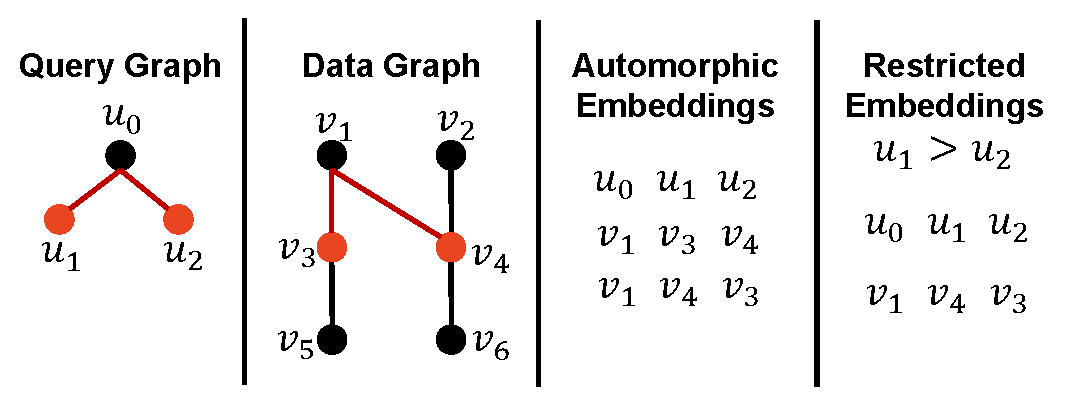
\includegraphics[width=\columnwidth]{./figure/automorphism.eps}
\caption{Examples of automorphic and non-automorphic embeddings.}	
\label{fig:automo}
\end{figure}

If a query graph is symmetric, multiple embeddings can be isomorphic to the same subgraph of a data graph. As shown in Figure \ref{fig:automo}, the query graph has two symmetric vertices, $u_1$ and $u_2$ and two isomorphic embeddings. We can see in Figure \ref{fig:automo} that the two embeddings are the same subgraph of the data graph. To eliminate redundant embeddings, GraphPi \cite{shi2020graphpi} and GraphZero \cite{mawhirter2019graphzero} generate restrictions on query vertices and the corresponding data vertices in each embedding. Figure \ref{fig:automo} shows that with the restriction $u_1 > u_2$, we can eliminate the redundant embedding. We use the same method as GraphPi and GraphZero to break the symmetry of a query graph.

\subsection{GPU Architecture}
GPUs are general-purpose massively parallel computing devices. They are widely used to accelerate graph processing tasks, including
subgraph matching \FIXME{\cite{}}. GPU processing units can be abstracted into a two-level hierarchy, the Streaming Multiprocessors (SMs)
and computing cores inside the SM. An SM is further divided into processing blocks. Each processing block contains a fixed number of
threads, called a warp that is the basic scheduling unit.

Modern GPUs also organize their memory into a hierarchical system, containing the global memory, a configurable shared memory, registers,
and potentially an L2 cache between the global memory and the shared memory. The thread-local registers are the fastest memory component,
having the lowest access latency (1-2 cycles). The SM local L1 caches and shared memory provide a larger storage capacity over the
thread-local registers but have modestly higher accessing latency of around 30 cycles. Like the RAM in a CPU system, the GPU’s off-chip
global memory provides the largest memory storage capacity on the GPU but has the most expensive accessing latency of around 500 cycles.

The NVIDIA CUDA programming model provides atomic functions to perform a read-modify-write atomic operation on one 32-bit or 64-bit word
residing in global or shared memory. In this work, we use the CUDA $atomicAdd$ function. This function reads a variable in global memory
before adding a number to it and then writes the result back to the same address.



%GPU has been used in many areas to accelerate applications. The popularity of GPU is primarily attributed to its massive parallelism. To support such large-scale parallelism, GPU employs a complex execution pipeline and memory hierarchy. Modern GPUs usually consist of multiple Streaming Multiprocessors (SMs), and each SM contains multiple Single-Instruction-Multiple-Thread (SIMT) units. Threads in the same SIMT unit are called a warp, the smallest scheduling unit in GPU. The thread-local registers are the fastest memory component, having the lowest access latency (1-2 cycles). The SM local L1 caches and shared memory provide a larger storage capacity over the thread- local registers but have modestly higher accessing latency of around 30 cycles. The off-chip global memory, similar to the RAM in a CPU system, provides the largest memory storage capacity on the GPU but has the longest accessing latency of around 500 cycles.
%
%CUDA provides atomic functions to perform a read-modify-write atomic operation on one 32-bit or 64-bit word residing in global or shared memory. In this work, we use $atomicAdd$ function to read a variable in global memory and add a number to it, and write the result back to the same address.

\section{Related Work}
\subsection{CPU-based Subgraph Matching}
An early attempt for subgraph matching is Ullmann \cite{ullmann1976algorithm}. They use a tree-search based approach to mine subgraphs and a look-ahead function to prune search space. Many works \cite{cordella2001improved, shang2008taming,zhang2009gaddi,he2008graphs,zhao2010graph} based on Ullmann have been proposed. VF2 \cite{cordella2001improved} uses degree information of vertices to prune the search space further. QuickSI \cite{shang2008taming} proposes to match vertices that have infrequent vertex and edge labels to eliminate invalid embeddings as early as possible. GADDI \cite{zhang2009gaddi}, GraphQL \cite{he2008graphs}, and SPath \cite{zhao2010graph} utilize the neighborhood information to remove unqualified data vertices from the candidate set for each query vertex. CECI \cite{bhattarai2019ceci} proposes a compact embedding cluster index to divide the data graph into embedding clusters and conduct subgraph matching on each embedding cluster. The main focus of these algorithms is to reduce the size of candidate sets. They do not take into account the impact of the matching order of query vertices on the matching performance, as pointed out in \cite{lee2012depth}.

In order to further improve the performance of subgraph matching, subsequent works \cite{han2013turboiso,ren2015exploiting,bi2016efficient,han2019efficient,rivero2017efficient} try to build auxiliary data to devise an effective matching order. TurboIso \cite{han2013turboiso} first identifies candidate regions in a data graph and then generates a matching order for each candidate region based on the number of candidate vertices of query vertices in this candidate region. BoostIso \cite{ren2015exploiting} exploits relationships between vertices in a data graph to remove duplicate computations. CFL \cite{bi2016efficient} decomposes the query graph into the core-forest-leaf structure and matches the core structure first to eliminate invalid embeddings as early as possible. Han et al. \cite{han2019efficient} builds a directed acyclic graph (DAG) for a query graph and then generates a matching order based on the DAG. SGMatch \cite{rivero2017efficient} decomposes the query graph into graphlets and then generates a matching order based on graphlets.

In recent years, many parallel subgraph matching algorithms have emerged.  Distributed subgraph matching  has been explored in \cite{afrati2013enumerating, shao2014parallel,shi2020graphpi,talukder2016distributed,sun2018parallelizing,plantenga2013inexact,reza2018prunejuice}. These approaches use MPI and MapReduce to distribute subgraph matching tasks to different compute nodes.

Different from CPU-based approaches, our work focuses on exploiting a GPU's massive parallelism to match a query graph in a data graph.

\subsection{GPU-based Subgraph Matching}
GPU has been used to accelerate applications in many fields because of its massive parallelism. There are several works exploiting GPU acceleration for subgraph matching. TRICORE \cite{hu2018tricore}  and \cite{green2014fast} design a GPU-based triangle counting method. Guo at el. \cite{guo2020gpu} partitions the data graph that beyond the GPU memory into subgraphs and matches the query graph in each subgraph iteratively. They also propose an embedding reuse method to avoid repeated computation in the work \cite{guo2020exploiting}. GSI \cite{zeng2020gsi}, GSM \cite{wang2020fast}, GpSM \cite{tran2015fast}, and \cite{lin2016network} utilize auxiliary data to assist candidate pruning and some GPU-based optimization techniques to speed up the matching process. While these works adopt the single-vertex extension method, our approach uses the double-vertex extension method to reduce the number of read and write operations of partial embeddings.



\section{Overview of Our Approach}
\begin{figure*}
	\centering
	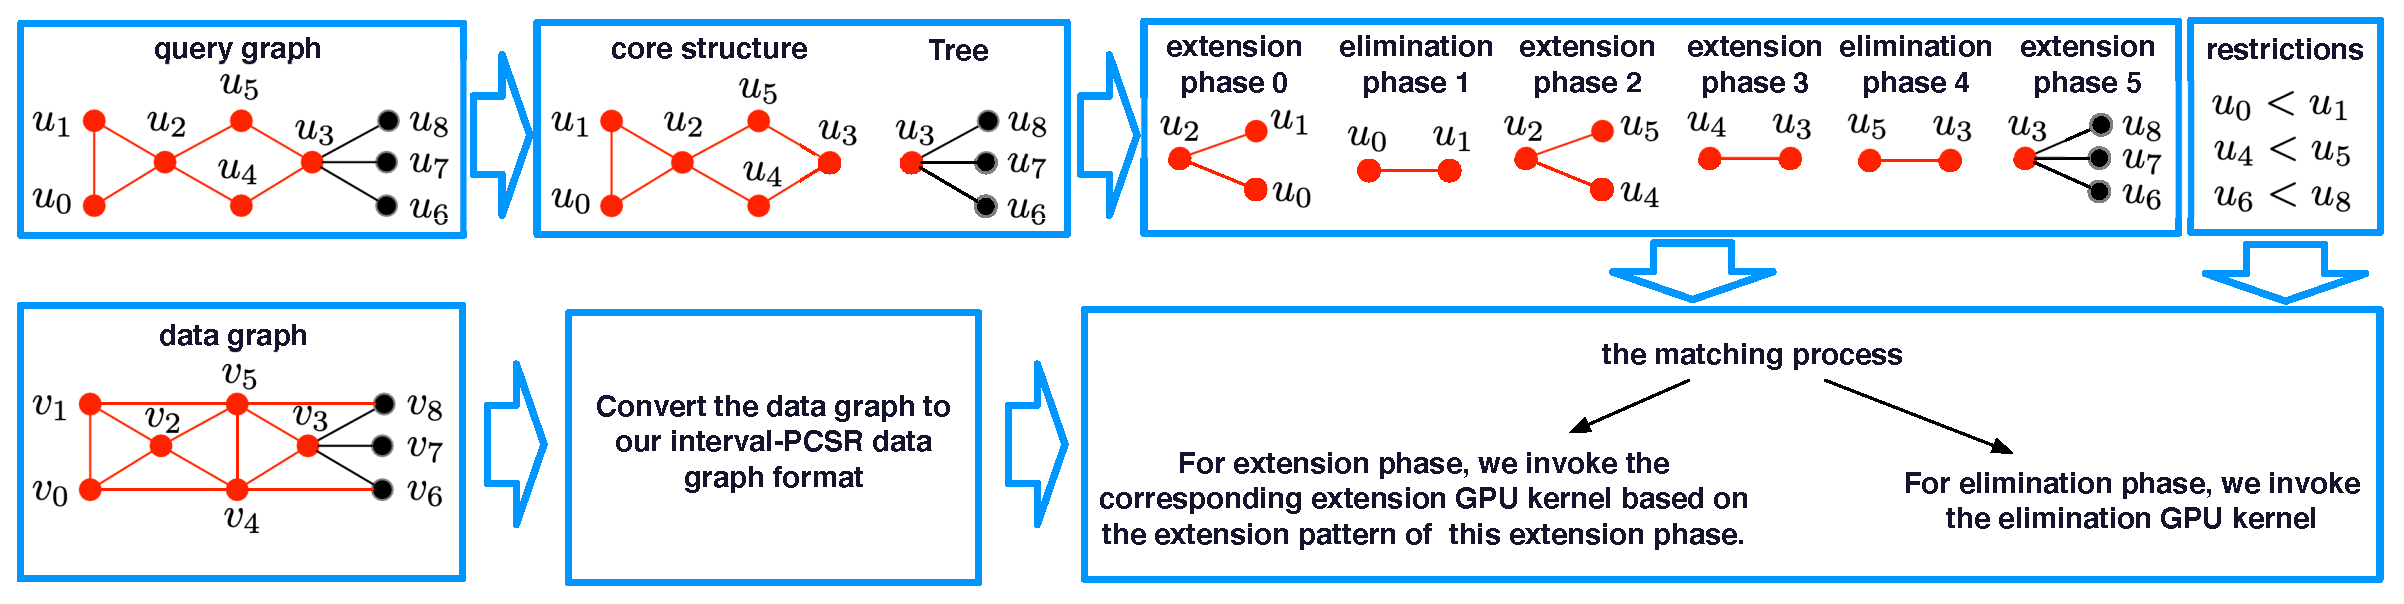
\includegraphics[width=\textwidth]{./figure/approachoverview.eps}
	\caption{An overview of our parallel vertex matching approach, \SystemName.}
	\label{fig:overview}
\end{figure*}

Figure~\ref{fig:overview} depicts the overall workflow of \SystemName. At the offline stage, we convert the data graph into a carefully designed storage format. This format is designed to accelerate GPU kernel computation while reducing the GPU memory footprint when processing large graphs (Section \ref{sec:storage}). We note that this storage conversion only needs to be performed once, which is a one-off cost performed offline.

During runtime, Algorithm \ref{algo:submatch} is used to perform subgraph search. We first decompose the query graph into the core structure and trees according to the method proposed in \cite{bi2016efficient}, and further decompose them into extension and elimination phases. Each extension phase contains exactly one matching pattern shown in Figure \ref{fig:matchpattern} and each elimination phase contains one or more non-tree edges. In the meanwhile, we generate a matching order for extension and elimination phases, and restrictions on query vertices (line 1). All edges in an extension or elimination phase have the same edge label since we load one edge label partition at each iteration (lines 2, 7). The first extension phase of the matching order is used to generate initial embeddings (line 4). The main difference between the first and following extension phases is that the source vertices of the former one are from the edge label partition, while the later one are from previous embeddings. Finally, we use different GPU kernels to handle extension and elimination phases (lines 10, 12), and output final embeddings (line 13). In the following sections, we elaborate each step in detail.


\section{Data Graph Storage Format\label{sec:storage}}
\begin{figure*}
\centering
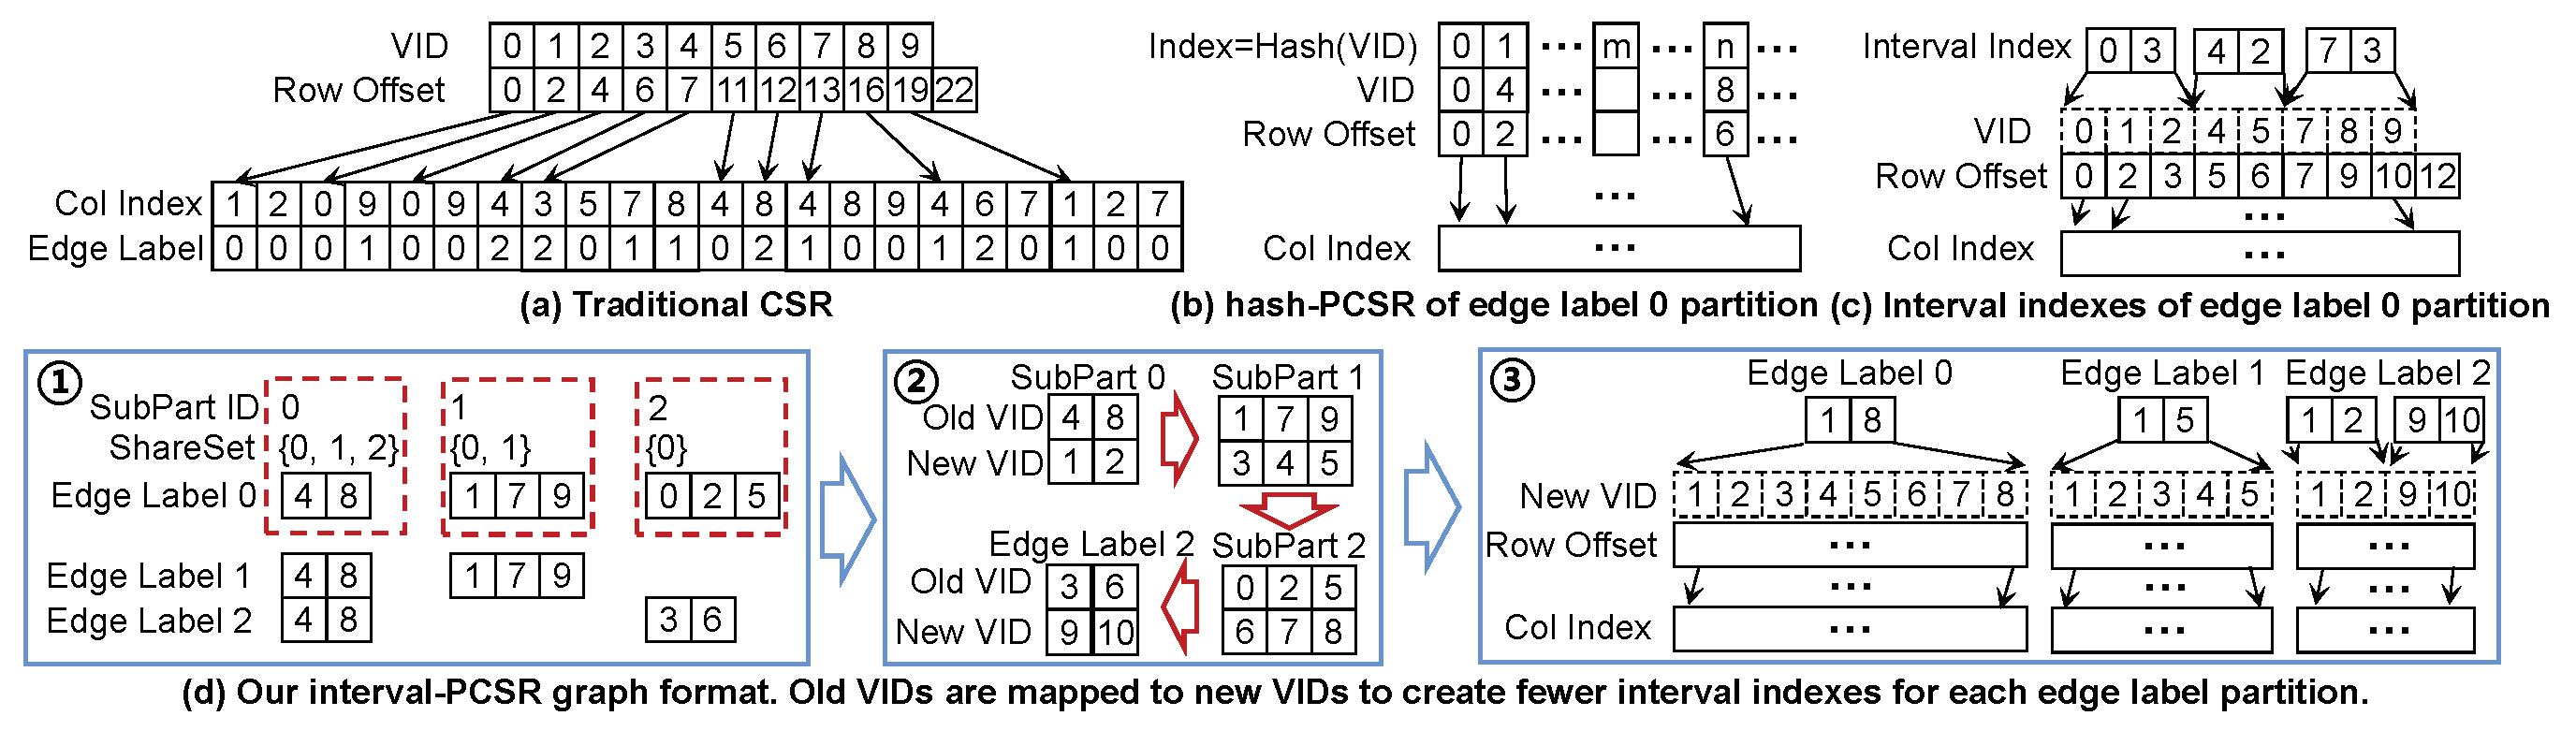
\includegraphics[width=\textwidth]{./figure/graphformat.eps}
\caption{Demonstration of data graph formats generated by traditional CSR (a), hash-PCSR that is used by GSI (b), non-optimized interval-PCSR (c), and our
optimized interval-PCSR (d). Note that VIDs in dashed squares do not need to be stored in memory.}	
\label{fig:dataformat}
\end{figure*}


\begin{algorithm}[t!]
\KwIn{the data graph in our format $G$, the query graph $q$} \KwOut{Embeddings of $q$ $EMB$} $\pi \leftarrow \textsc{GenMatchOrder}(q)$\;
Load the edge label partition $elp$ whose edge label is $\pi[0].edgeLabel$ from $G$ to GPU\; Allocate all available GPU memory space to
$newEMB$\; $\textsc{ExtKernel}(elp,NULL,newEMB,\pi[0])$\; $EMB \leftarrow newEMB$\; \For{$i \leftarrow 1$ \KwTo $\pi .size$}{
	Load the edge label partition $elp$ whose edge label is $\pi[i].edgeLabel$ from $G$ to GPU\;
	Allocate all available GPU memory space to $newEMB$\;
	\If{$\pi[i]$ is an extension phase}{
		$\textsc{ExtGPUKernel}(elp,EMB,newEMB,\pi[i])$\;
	}
	\Else{
		$\textsc{EliGPUKernel}(elp,EMB,newEMB,\pi[i])$\;
	}
	$EMB \leftarrow newEMB$\;
} \caption{\textsc{SubgraphSearch}} \label{algo:submatch}
\end{algorithm}

Real-world graphs are often too large to fit into the memory of a single GPU. Therefore, only part of the data that is needed for the
current computation should be stored in the GPU memory at a given time. As a result, it is important to find a compact representation of
the graph data without compromising the computation performance. To this end, \SystemName extends the Partitioned Compressed Sparse Row
(PCSR), the data graph storage format used by GSI \cite{zeng2020gsi}. This format groups edge with the same label into an edge label partition,
which is then stored in the Compressed Sparse Row (CSR) sparse matrix storage format. By doing so, only the partition with
the same edge label as the matching edge needs to be moved from the CPU memory into the GPU memory. PCSR makes some small modifications to
the CSR format. As depicted in Figure \ref{fig:dataformat}a, a vertex ID (VID) can be used to find the row offset of a vertex because VIDs are stored
as contiguous elements in a classical CSR. Because after grouping edges into partitions, VIDs of vertices are no longer guaranteed to be
continuous in the storage space, GSI employs a hash function to translate a VID into a slot the corresponding elements in the edge partition structure. To reduce collisions of the hash function, some empty entries have to be reserved
for each vertex (30 in GSI), which results in a large portion of unused GPU memory space. \SystemName is designed to avoid this pitfall.


\subsection{\SystemName Data Graph Storage Format}

\begin{algorithm}[t!]
\KwIn{the set of all edge label partitions $ELP$}
\KwOut{the mapping array $MAP$ with old and new VIDs are indices and values respectively}	
$newVID \leftarrow 1$\;
\While{ $ELP \neq \emptyset$ }{
	Choose the partition $elp \in ELP$ that has the most vertices\;
	Divide $elp$ into sub-partitions $subParts$\;
	\ForEach{$subPart \in subParts$}{
		Group IDs of partitions that contain $subPart$ into $shareSet$ and delete vertices of $subPart$ from these partitions\;
	}
	\While{$subParts \neq \emptyset$}{
		Choose the $subPart \in subParts$ that is shared by the most partitions and delete it from $subParts$\;
		Construct $MAP$ (assign new vertex IDs starting from $newVID$ to vertices in $subPart$ contiguously)\;
		$newVID \leftarrow newVID + subPart.size$\;
		$preSubPart \leftarrow subPart$\;
		\While{$preSubPart \neq \emptyset$}{
			Choose the $subPart \in subParts$ whose $shareSet$ has the most same partition IDs with the $shareSet$ of $preSubPart$ and delete the $subPart$ from $subParts$\;
			\If{Found the $subPart$}{
				Construct $MAP$\;
				$newVID \leftarrow newVID + subPart.size$\;
				$preSubPart \leftarrow subPart$\;
			}
			\Else{
				$preSubPart \leftarrow \emptyset$\;
				break\;
			}
		}
	}
	$ELP \leftarrow ELP/elp$\;
}
\caption{\textsc{GenMap}}
\label{algo:genmap}
\end{algorithm}

To reduce the amount of unused memory space required by the PCSR's hash function, we record the range of contiguous VIDs of an edge label
partition (ELP). The contiguous range of VIDs is recorded in an \emph{interval index} structure as shown in Figure \ref{fig:dataformat}c,
which stores the first VID and the number of continuous VIDs in the range.

Because an ELP may contain many small intervals, directly mapping each interval to be stored in an interval index will result in many
interval indices. This is not ideal because having a large number of interval indices means we will need many memory accesses to just find
the interval for a VID. For example, if we want to find the index of VID 7 in Figure \ref{fig:dataformat}c, with a naïve interval scheme,
we will have to compare number 7 against the first three interval indices before locating VID 7 in the third interval index. Our design
avoids this pitfall by carefully mapping the original VIDs to new VIDs, to allow one to generate more contiguous new VIDs in each edge
label partition, which in turn leads to a smaller number of intervals. Our data storage format shares the same spirit of Huffman coding \cite{Moffat2019Huffman} – we want to reduce the number of memory access when processing the largest ELP (i.e., the partition that contains the largest number of VIDs).

\subsection{\SystemName Storage Format Algorithm}

 As described in Algorithm \ref{algo:genmap} and Figure \ref{fig:dataformat}d, \SystemName takes several steps to convert the data graph into a GPU-tuned storage format, described as follows.

\cparagraph{Step 1: Find the largest ELP.} We start by choosing the partition that contains the most vertices (line 3 in Algorithm
\ref{algo:genmap}). Our intuition is that the more vertices a partition contains, the higher probability it will be accessed. Therefore,
reducing the number of intervals for this partition can help reduce the average memory access latency. For the example shown in Figure
\ref{fig:dataformat}d \textbf{\textcircled{1}}, edge label partition 0 is selected because it contains the largest number of vertices.

\cparagraph{Step 2: Rename VIDs.} In the second step, we try to increase the continuous VID interval by renaming the VIDs. To this end, for
each vertex, we find out all ELPs that contain the vertex. For example, vertices 4 and 8 in Figure \ref{fig:dataformat}d \textbf{\textcircled{1}} belong to ELPs 0,
1 and 2 - these ELPs form a share set for the two vertices. Next, we merge VIDs that have the same shares set into a subpartition (line 4
in Algorithm~\ref{algo:genmap}). For the example shown in Figure \ref{fig:dataformat}d \textbf{\textcircled{1}}, we map vertices 4 and 8 to a subpartition, subpart 0, because they have the same share set. We apply this grouping strategy to the largest ELP found in step 1. For the vertices that belong
to the same subpartition, we can assign unique, continuous new VIDs to them in arbitrary order, as long as these new VIDs are contiguous
and follow the largest VID from the last processed subpartition.

\cparagraph{Step 3: Process subpartitions.} To determine the order of the subpartitions of an ELP to be processed, we start from the
subpartition that is shared by most ELPs.  This means for the example shown in Figure \ref{fig:dataformat}d \textbf{\textcircled{1}}, we would first process
subpart 0, because it has the largest share set (with 3 ELPs).  The next subpartition we choose will be the one that has the largest number of common ELPs between its share set and the shared set of the last chosen subpartition. Looking at Figure \ref{fig:dataformat}d \textbf{\textcircled{1}} again, subpartition 1 will be the secondly chosen subpartition because its shared set has two ELPs ($0, 1$) with the share set of subpartition 0 (the firstly chosen subpartition). We choose this strategy because of the following two reasons.
First, the larger number of elements in common in the shared sets of two subpartitions, the more ELPs will have the two subpartitions.
Secondly, because we ensure the VIDs between two consecutively processed subpartitions are continuous, we can then merge the VIDs of the
two subpartitions to form a contiguous interval to be stored in a single interval index. Using this strategy, we can use a single interval index to record the new VIDs of subpartitions 0 and 1 in Figure \ref{fig:dataformat}d \textbf{\textcircled{2}}.


\cparagraph{Step 4: Repeat before Stop.} We delete the processed vertices from an ELP, and repeat steps 1 to 4 for each ELP in turn. This
process stops until all VIDs have been renamed and recored in the interval indices. This is illustrated in Figure \ref{fig:dataformat}d \textbf{\textcircled{3}}.


Figure \ref{fig:dataformat} shows the storage size of \SystemName against the PCSR scheme used by GSI for eight data graphs. The \SystemName storage
format reduces the storage size (and the GPU memory footprint) by 83\%.

\section{Extension and Elimination\label{sec:extensionphase}}
Like mainstream graph matching frameworks \cite{tran2015fast, zeng2020gsi}, \SystemName applies a two-step approach to perform graph
search. In the extension phase, \SystemName matches graph vertices and edge labels between the query and the data graph to generate embeddings (i.e., matched subgraphs). In the elimination phase, we remove embeddings that do not match the specified non-tree query edges.


\subsection{The Extension Phase}

For a given query graph and a data graph in the \SystemName storage format, we iteratively perform subgraph matching in multiple extension
phases. Each extension phase processes one of the matching patterns depicted in Figure \ref {fig:matchpattern}. Previous works
\cite{zeng2020gsi,sun2020subgraph} use the traditional single vertex matching (SV-match) scheme. This scheme requires extensive load and
store operations to the GPU memory because it needs to write the intermediate results after matching a query vertex and read the same
intermediate results before matching the next query vertex. \SystemName is designed to avoid this pitfall.


A key hurdle for performing subgraph search on GPUs is that the number of embeddings generated by a GPU warp (the basic
GPU scheduling unit – see Section \ref {sec:gpu}) is different, and we have to carefully compute the memory location
used to store the newly generated embeddings for each warp to avoid write conflicts. Prior works address this problem
by either generating the embeddings twice (in order to use the first generation to compute the store locations)
\cite{tran2015fast} or need to access all embeddings twice to compute the store location \cite{zeng2020gsi}.
\SystemName takes a different approach by utilizing the CUDA \texttt{atomicAdd} primitive inside the extension kernel
to directly compute the write addresses across GPU wraps, eliminating the need of accessing or generating an embedding
twice. This atomic instruction ensures only one wrap can update the same variable at any given time and hence avoids
the race condition of determining the store location of the embeddings across wraps. While there is an overhead
associated with \texttt{atomicAdd}, we found that this is not a severe problem in subgraph search because of the
intrinsic irregularity of graph structures.

\begin{algorithm}[t]
\KwIn{the edge label partition $elp$, partial embeddings $EMB$, the starting address of new embeddings $newEMB$, the extension phase
$extP$} $totNum \leftarrow 0$\; Load interval indexes of $elp$ into shared memory\; \ForEach{$emb \in EMB$}{
	Get source VIDs $u_{s1}$ and $u_{s2}$ from $emb$\;
	Search $u_{s1}$ and $u_{s2}$ in interval indexes and extract their neighbors $ne1$ and $ne2$, respectively.\;
	Remove neighbors that do not have the same vertex labels as $u_{1}$ and $u_{2}$ from $ne1$ and $ne2$, respectively\;
	Remove neighbors that do not satisfy the restrictions of $u_{1}$ and $u_{2}$ from $ne1$ and $ne2$, respectively\;
	\If{$extP$ is matching pattern 0}{
		We use the traditional SV-ext method to generate embeddings for $extP$\;
	}
	\ElseIf{$extP$ is matching pattern 1}{
		$\textsc{OptDouExt}(emb,ne1,totNum,newEMB)$\;
	}
	\ElseIf{$extP$ is one of matching patterns 2, 3, and 4}{
		$\textsc{DouExt}(emb,ne1,ne2,totNum,newEMB)$\;
	}
	\ElseIf{$extP$ is one of matching patterns 5, 6, and 7}{
		$\textsc{NExt}(emb,ne1,ne2,totNum,newEMB,extP)$\;
	}
}

\caption{\textsc{ExtPhaseKernel}} \label{algo:extphase}
\end{algorithm}



Algorithm \ref{algo:extphase} describes the overall workflow of the \SystemName extension phase. For each embedding (line 3), we first
obtain the source VIDs from the embedding according to the matching pattern to be processed (line 4). Next, we search the source VIDs in
the \SystemName interval-PCSR of the loaded ELP and extract their neighbors (line 5).  Then, we remove invalid neighbors that either have wrong
vertex labels or do not satisfy the restrictions. Finally, we use different algorithms to generate new
embeddings for different matching patterns (lines 8-15).

In the remainder of this section, we first describe embedding generation methods for the fundamental matching patterns 2-4 of Figure
\ref{fig:matchpattern}. We then describe our optimized embedding generation method for the matching pattern 1 of Figure \ref{fig:matchpattern} before showing how our optimizations can be extended to matching patterns 5-7. The matching pattern 0 uses the tradition method to generate embeddings, thus we do not elaborate it in this work.

\subsection{Matching Patterns 2 to 4}

For matching patterns 2-4, we employ a simple method described in Algorithm \ref{algo:generalDV} to generate new
embeddings. Our key idea is to iterate over all combinations of candidates of $u_{1}$ and $u_{2}$ in the data graph
(denoted as $C_1$ and $C_2$ respectively) to construct new embeddings by appending each valid combination to a new copy
of the current embedding $emb$. We consider a combination to be valid if none of the VIDs in the combination \FIXME{is
presented in the current - check this}  $emb$. To avoid checking this condition repeatedly, we first check this
condition for all vertices in $C_2$ once (lines 3-4) and record indexes of vertices whose VIDs also exist in $emb$
(line 5). To fully utilize $C_2$, we generate new embeddings while checking the condition. Once a vertex in $C_2$ is
checked to be valid (lines 6-7), we assign this vertex and the first valid vertex in $C_1$ to $u_2$ and $u_1$,
respectively (lines 1,8). Then, we store the new embedding $(emb,u_1,u_2)$ to the corresponding address (lines 9-10).

\begin{algorithm}[t!]
	\KwIn{the partial embedding $emb$, candidates of $u_1$ $C_1$, candidates of $u_2$ $C_2$, the number of newly written embeddings $totNum$, the starting address of new embeddings $newEMB$}
	Find the index $i$ of the first valid vertex in $ne1$\;
	$writePos \leftarrow atomicAdd(totNum,1 \times C_{2}.size)$\;
	\For{$j \leftarrow 0$ \KwTo $C_{2}.size$}{
		\If{$C_2[j] \in emb$}{
			Add $j$ to the set $boundry$\;
			$u_1 \leftarrow 0$; $u_2 \leftarrow 0$\;
		}
		\Else{
			$u_1 \leftarrow C_1[i]$; $u_2 \leftarrow C_2[j]$\;
		}
		Write the new embedding ($emb$, $u_1$, $u_2$) to the address pointed by $newEMB+writePos$\;
		$writePos \leftarrow writePos + emb.size+2$\;
	}
	$i \leftarrow i+1$\;
	\While{$i < C_{1}.size$}{
		Load 32 candidates from $C_1$ into $tmp$; $i \leftarrow i+32$\;
		Remove candidates that exist in $emb$ from $tmp$\;
		$writePos \leftarrow atomicAdd(totNum,tmp.size \times (C_{2}.size-boundry.size))$\;
		\ForEach{$0 \leq k<tmp.size$ and $0 \leq j<C_{2}.size$ and $j \notin boundry$}{
			\If{This is EP 2 and $C_1[k]=C_2[j]$}{
				$u_1 \leftarrow 0$; $u_2 \leftarrow 0$\;
			}
			\Else{
				$u_1 \leftarrow C_1[k]$; $u_2 \leftarrow C_2[j]$\;
			}
			Write the new embedding ($emb$, $u_1$, $u_2$) to the address pointed by $newEMB+writePos$\;
			$writePos \leftarrow writePos + emb.size+2$\;
		}
	}
	\caption{\textsc{DouExt}}
	\label{algo:generalDV}
\end{algorithm}

At the beginning of Algorithm \ref{algo:generalDV}, we allocate space for new embeddings generated when checking
conditions for $C_2$ (line 2). Since we do not know the number of valid vertices in $C_2$ ahead of time, we allocate
space to store the maximum sized embedding – the number of vertices in  $C_2$ (denoted as $C_{2}.size$). If there are
invalid vertices in $C_2$, we assign 0 to $u_1$ and $u_2$ to indicate invalid embeddings (line 6). During processing,
the GPU kernel then ignores embeddings that contains a zero.


In Algorithm \ref{algo:generalDV}, after finding invalid vertices in $C_2$, we generate new embeddings for the rest
vertices in $C_1$ (lines 11-12). In each iteration, we load 32 vertices in $C_1$ into the shared memory buffer $tmp$
and remove invalid ones from it (lines 13-14). To allocate space for new embeddings, we estimate its count as the
number of combinations of $tmp$ and valid vertices in $C_2$ (line 15). Then, we generate new embeddings for these
combinations (line 16). As $u_1$ and $u_2$ have the same vertex label in extension pattern 2, it is possible that two
candidates of $u_1$ and $u_2$ are identical (line 17),  leading to an invalid new embedding. To solve the problem, we
assign 0 to $u_1$ and $u_2$ if the embedding is invalid (line 18); otherwise, we assign the corresponding candidates to
$u_1$ and $u_2$ (line 20). Finally, we store the new embedding to the specified address (lines 21-22).


\subsection{Matching Pattern 1}
\begin{figure} [t]
\centering
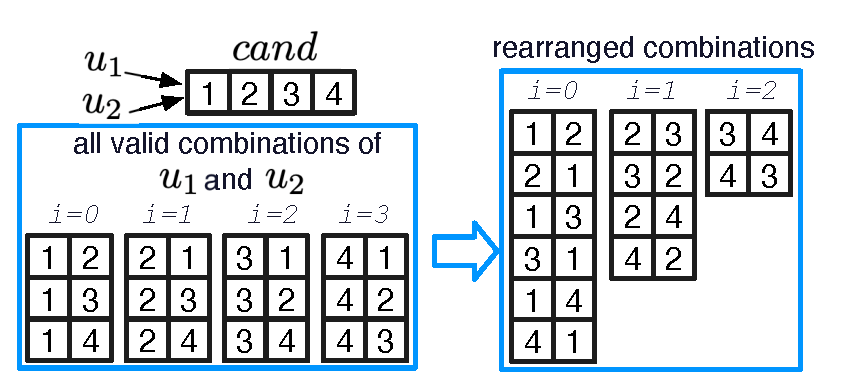
\includegraphics[width=\columnwidth]{./figure/ep1opt.eps}
\caption{An example of generating new embeddings for the matching pattern 1.}	
\label{fig:ep1opt}
\end{figure}


\begin{algorithm}[t]
	\KwIn{embeddings $emb$, candidates $C$, the number of newly written embeddings $totNum$, the starting address of new embeddings $newEMB$}
	$writePos \leftarrow atomicAdd(totNum,C.size \times (C.size-1))$\;
	\For{$i \leftarrow 0$ \KwTo $C.size-1$}{
		\For{$j \leftarrow i+1$ \KwTo $C.size$}{
			Write new embeddings ($emb$, $C[i]$, $C[j]$) and ($emb$, $C[j]$, $C[i]$) to the address pointed by $newEMB+writePos$\;
			$writePos \leftarrow writePos + (emb.size+2) \times 2$\;
		}
	}
	\caption{\textsc{OptDouExt}}
	\label{algo:optDV}
\end{algorithm}
Algorithm \ref{algo:generalDV} is ill-suite for matching pattern 1. For this matching pattern, $u_1$ and $u_2$ are extended from the same
source vertex $u_{s1}$ and have the same vertex label, i.e., $C_1 = C_2$. If Algorithm \ref{algo:generalDV} is applied to this pattern,
each vertex in $C_2$ can be accessed by up to $C_1.size$ times. As shown in the left part of Figure \ref{fig:ep1opt}, element 1 is accessed
at each iteration of $i$. If $C_1.size>32$, we need to reload element 1 from global memory each time we access it. Aceesing other elements
also have the same problem.

\SystemName is designed to accelerate the matching process of matching pattern 1. We achieve this by rearranging the generation order of
combinations, as shown in \FIXME{Figure \ref{fig:ep1opt} b}. This arrangement promotes register usage, which in turn reduces the memory
accessing latency. The core design of our optimized generation method for matching pattern 1 is shown in Algorithm \ref{algo:optDV}. From
\FIXME{Figure \ref{fig:ep1opt} b}, we make two important observations to guide the design of Algorithm \ref{algo:optDV}. First, since the
element $C_1[i]$ is only used at iteration $i$, we will load it into a register (line 2) to reduce its access latency. Second, each time we
generate a combination, we can reverse the combination to obtain another combination immediately without reloading data from global memory
(lines 4-5).



\subsection{Matching Patterns 5 to 7}
\begin{algorithm}[t!]
	\KwIn{embeddings $emb$, candidates of \{$u_1, \cdots, u_n$\} $C_1$, candidates of \{$u_{n+1}, \cdots, u_{n+m}$\} $C_2$, the number of newly written embeddings $totNum$, the starting address of new embeddings $newEMB$, extension phase $extP$}
	\If{$extP$ is matching pattern 5}{
		\ForEach{$comb1$ of combinations of $u_1, \cdots, u_{n-2}$}{
			$emb_{copy} \leftarrow (emb, comb1)$; $C_{copy} \leftarrow C_1/comb1$\;
			$\textsc{OptDouExt}(emb_{copy},C_{copy},totNum,newEMB)$\;
		}
	}
	\ElseIf{$extP$ is one of matching patterns 6 and 7}{
		\ForEach{$comb2$ of combinations of $u_{n+1}, \cdots, u_{n+m}$}{
			\ForEach{$comb1$ of combinations of $u_1, \cdots, u_{n-2}$}{
				$emb_{copy} \leftarrow (emb, comb1, comb2)$; $C_{copy} \leftarrow C_1/comb1$\;
				$\textsc{OptDouExt}(emb_{copy},C_{copy},totNum,newEMB)$\;
			}
		}
	}
	\caption{\textsc{NExt}}
	\label{algo:nvext}
\end{algorithm}

Our approach for generate embeddings for matching patterns 5-7 is described in Algorithm \ref{algo:nvext}, which extends Algorithm
\ref{algo:optDV}. For matching pattern 5 (line 1), we iterate over all combinations of $u_1, \cdots, u_{n-2}$ (line 2) and use Algorithm
\ref{algo:optDV} to match the last two query vertices $u_{n-1}$ and $u_n$ (line 4). Before invoking Algorithm \ref{algo:optDV}, we need to
construct a new embedding and new candidates for $u_{n-1}$ and $u_n$ (line 3). For matching patterns 6 and 7, we first use an outer loop to
iterate over all combinations of $u_{n+1}, \cdots, u_{n+m}$, and use the same method as the matching pattern 5 to generate embeddings
(lines 7-9).


\subsection{Priorities of Matching Patterns}
When decomposing the query graph into extension and elimination phases, there is a possibility that multiple matching patterns are available for an extension phase. To choose the most suitable matching pattern, we assign 2-level priorities to matching patterns. In the first level, we prioritize matching patterns based on the number of query vertices to be matched in each matching pattern. Thus, matching patterns 5-7 get the highest priority, 1-4 get the medium priority, and 0 gets the lowest priority. In the second level, we prioritize matching patterns that posses the same first level priority based on efficiency of each matching pattern when generating embeddings.

We first analyze the efficiency of medium priority matching patterns, and then the highest priority ones. The matching pattern 1 uses an optimized method (Algorithm \ref{algo:optDV}) to generate embeddings, thus it is most efficient among matching patterns 1-4. matching patterns 2-4 use the normal method (Algorithm \ref{algo:generalDV}) but the matching pattern 2 needs to evaluate the equality of candidates of $u_1$ and $u_2$. Therefore, the matching pattern 2 is the least efficient one. Compared to the matching pattern 3, the matching pattern 4 needs one more step to find the address of $u_{s2}$, thus it is less efficient than the matching pattern 3. Consequently, the priority order of matching patterns 1-4 from the highest to the lowest is matching pattern 1, 3, 4, and 2.

Among matching patterns of the highest priority, the matching pattern 5 is the most efficient one because it only needs one step to find the neighbor address of $u_{s1}$ in the edge label partition and another step to find the address of neighbors that have the same vertex label as $u_1, \cdots, u_n$. In contrast, the matching pattern 7 is the least efficient one because it needs one more step to find the neighbor address of $u_{s2}$ compared to the matching pattern 5. Consequently, the priority order of matching patterns 5-7 from the highest to the lowest is matching pattern 5, 6, and 7.


\subsection{The Elimination Phase\label{sec:eliphase}}
In the elimination stage, \SystemName removes illegible embeddings that do not match the specified non-tree query edges. As shown in Figure \ref{fig:overview}\textbf{\textcircled{2}}, the embedding $(v_1, v_4, v_0)$ is removed because there is no edge between $v_4$ and $v_0$ that can match the query edge $(u_0, u_1)$.

GSI \cite{zeng2020gsi} matches only one query edge in a GPU kernel and Lai et al. \cite{lai2015scalable} matches at most two query edges at
each iteration. Both methods can not fully utilize the elimination power of non-tree edges. In our approach, we match as many non-tree
edges as possible to eliminate invalid embeddings at early stages. Algorithm \ref{algo:eliphase} demonstrates how our approach deals with
the eliminate phase. For each embedding $emb$ (line 2), we first check if all query edges in the elimination phase can be matched in $emb$
(line 4). If so (line 5), we write $emb$ to the shared memory $tmp$ (line 6) and write $tmp$ to global memory if it is full (lines 7-9).


\begin{algorithm}[t!]
\KwIn{the edge label partition $elp$, embeddings $EMB$, the number of generted embeddings $totNum$, the elimination phase $eliPhase$}
Load interval indexes of $elp$ into shared memory\;
\ForEach{$emb \in EMB$}{
	\ForEach{$edge \in eliPhase$}{
		Check if there is an edge in $emb$ that can match $edge$\;
	}
	\If{all edges in $eliPhase$ are matched}{
		Write $emb$ to shared memory $tmp$\;
		\If{$tmp$ is full}{
			$writePos \leftarrow atomicAdd(totNum,tmp.size)$\;
			Write $tmp$ to the address pointed by $newEMB+writePos$\;
		}
	}
}
\caption{\textsc{EliPhaseKernel}}
\label{algo:eliphase}
\end{algorithm}


%\subsection{Matching and Work Scheduling}

\section{Matching Order\label{sec:matchingorder}}
We use the same method as \cite{bi2016efficient} to decompose the query graph into the core structure and trees, as shown in Figure \ref{fig:overview}. We also match the core structure first, and then the trees. The main difference is that our approach is designed specifically for parallel vertex matching.

When decomposing the core structure into extension and elimination phases, we need to adhere to an important constraint, which is that only matching patterns 0-4 can be used to decompose the core structure. The reason is explained as follows. In order to eliminate invalid embeddings as soon as possible, we need to first match circles in the core structure like $\{u_0, u_1, u_2\}$ in Figure \ref{fig:overview}. Therefore, we only need to match at most two vertices when matching a circle because vertices in a circle have exactly two neighbors. Figure \ref{fig:overview} demonstrates that the core structure is decomposed into matching patterns 0 and 1. We can see in the core structure that $u_0$, $u_1$, $u_2$, and $u_3$ can be matched with the matching pattern 6 where $u_2$ is the source vertex. If we first decompose the core structure with the matching pattern 6, and then the non-tree edge $(u_0, u_1)$, a large number of invalid embeddings may be generated, which significantly slows down the matching performance. After matching the core structure, we can use any appropriate matching patters to match trees. For example, the matching pattern 6 can be used to match the tree in Figure \ref{fig:overview}.


Based on \cite{bi2016efficient} and our parallel vertex matching method, we design Algorithm \ref{algo:genmatchorder} to generate matching order of extension and elimination phases. At the beginning of Algorithm \ref{algo:genmatchorder}, we adopt methods proposed in \cite{shi2020graphpi,mawhirter2019graphzero} to generate restrictions on VIDs in embeddings (line 1). Thus, we can avoid generating automorphic embeddings. Then we generate the core structure of $q$ by iteratively removing degree-one vertices from $q$, and construct trees of $q$ using removed vertices (line 2).

In order to match the core structure, we first find the smallest circle in the core structure (line 3), and then select vertices in the circle that conform to the highest priority matching pattern among matching patterns 0, 1, and 3 (line 4). The selected vertices constitute the first extension phase (lines 5-6), which is a special kind of extension phase. Different from the normal extension phase that fetches source vertices from embeddings (Figure \ref{fig:overview}\textbf{\textcircled{3}}), the first extension phase fetches the source vertex from the edge label partition (Figure \ref{fig:overview}\textbf{\textcircled{1}}). After generating the initial phase, we iteratively find vertices in the circle that conform to matching patterns 0-4 and choose the one with the highest priority (lines 7-9). Finally, we use the non-tree edge in the circle to construct an elimination phase (line 10).

After decomposing the smallest circle, we iteratively construct extension and elimination phases for the rest vertices and edges in the core structure (line 11). First, we find all non-tree edges and group them by the edge label (lines 12-13). For each group, we construct an elimination phase (lines 14-15). If no non-tree edges are found, we search for unmatched vertices in the core structure that can form one of matching patterns 0-4, and choose the one with the highest priority (lines 16-18).

After matching the core structure, we can use any appropriate matching patterns in Figure~\ref{fig:matchpattern} to match rest vertices that are not in the core structure since there is no non-tree edge left. At each iteration, we find vertices that can form matching patterns 0-7 and select the one with the highest priority (lines 19-21).


\begin{algorithm}
	\KwIn{the query graph $q$}
	\KwOut{the match phase queue $matchPhase$}
	Generate restrictions to eliminate automorphisms\;
	Generate the core structure $C$ and trees $T$ of $q$\;
	Find the smallest circle $minc$ in $C$\;
	Select vertices in $minc$ that conform to matching patterns 0, 1, and 3, and choose the highest priority matching pattern\;
	Construct the initial phase with vertices corresponding to the selected matching pattern\;
	Add the initial phase to $matchPhase$\;
	\For{vertices in $minc$ that conform to matching patterns 0-4}{
		Choose the highest priority matching pattern and construct an extension phase\;
		Add the extension phase to $matchPhase$\;
	}
	Construct an elimination phase with the non-tree edge in $minc$ and add it to $matchPhase$\;
	\For{rest vertices and edges in $C$}{
		\If{there are non-tree edges}{
			Group all non-tree edges by the edge label\;
			\ForEach{group $g$}{
				Construct an elimination phase $eliPhase$ based on $g$ and add it to $matchPhase$\;
			}	
		}
		\Else{
			Find vertices that conform to matching patterns 0-4 and choose the one with the highest priority\;
			Construct an extension phase and add it to $matchPhase$\;
		}
	}
	\For{vertices in $T$}{
		Find vertices that can form matching patterns 0-7 and select the one with the highest priority\;
		Construct an extension phase and add it to $matchPhase$\;
	}
	\caption{\textsc{GenMatchOrder}}
	\label{algo:genmatchorder}
\end{algorithm}


%\subsubsection{Work Load Balance}
%\SystemName uses the maximum number of warps which can be concurrently active on a GPU to process all embeddings. In this way, a warp with a small workload can match the next embedding without waiting for other warps. Only when there are no embeddings left, the faster warps have to wait for the slower warps. Our approach is simple yet effective, it can mitigate load imbalance to some extend. \FIXME{Have no idea of what is talking about here. This is a naïve scheme and is not something that should be explicitly metioned}.

%In GPU, once a thread block is scheduled to run on an SM, it will not be scheduled out until all warps in this
%thread block are finished. Therefore, if one warp matches a vertex or an edge that has many candidates, all warps in the same thread block
%have to wait for its completion. To address this problem, GSI designs a four-layer balance scheme. However, their scheme needs to invoke a
%GPU kernel inside a GPU kernel, which is time-consuming as illustrated in Section \ref{sec:compargsi}. Different from GSI, we use fixed
%warps, which means that the maximum concurrent warps are generated and will not be scheduled out during execution, to perform subgraph
%search. In this way, a warp with small workload can match next embedding without waiting for other warps. Only when there is no embeddings
%left, the faster warps have to wait for the slower warps. Our approach is simple yet effective, it can mitigate load imbalance to some
%extend. A more powerful load balance scheme can be designed and we leave this for a future study.

\section{Experimental Results}


\subsection{Evaluation of Data Graph Formats}
In this section, we first present the space cost of three data graph formats, including CSR, hash-PCSR, and  interval-PCSR. The results are
shown in Table \ref{tab:graphsize}. We can see from Table \ref{tab:graphsize} that CSR has the smallest space among three data graph
formats. The reason is that all VIDs in CSR are contiguous and unique, while VIDs in PCSR are non-contiguous and many duplicate VIDs exist
in different edge label partitions. However, we need to transfer the whole CSR format graph to GPU in order to perform subgraph search,
which is space and time consuming. In contrast, our interval-PCSR achieves similar space cost as CSR but only needs to transfer one edge
label partition to GPU before each iteration of subgraph search. AS shown in Table \ref{tab:graphsize}, the size of the maximum edge label
partition in interval-PCSR (denoted as \emph{Max}) is greatly smaller than CSR, which makes data transfer in our approach more efficient.


\begin{table}
\centering
  \caption{Space cost of CSR, hash-PCSR, and interval-PCSR. The \emph{Max} column represents the size of maximum edge label partition in interval-PCSR. The \emph{reduce-hash} column represents the percentage of the saved space by interval-PCSR compared to hash-PCSR.}
  \label{tab:graphsize}
  \begin{tabular}{ccp{30pt}p{30pt}cp{30pt}}
  \hline
    Graph &CSR&interval-PCSR&hash-PCSR&\emph{Max}&\emph{reduce-hash}\\
    \hline
    Enron 		&1.6MB	&1.7MB	&13MB	&0.6MB	&87\% \\
    FirstMM 	&1.2MB	&1.5MB	&22MB	&0.5MB	&93\% \\
    DD 			&15MB	&11MB	&139MB	&2.1MB	&87\% \\
    Gowalla 	&8.1MB	&9.4MB	&74MB	&1.9MB	&94\% \\
    Patents 	&149MB	&184MB	&1.6GB	&26MB	&89\% \\
    Reddit 		&60MB	&71MB	&901MB	&10MB	&92\% \\
    Orkut 		&906MB	&997MB	&1.94GB	&100MB	&50\% \\
    sinaweibo	&2.2GB	&2.5GB	&10GB	&256MB	&75\% \\

    \hline
  \end{tabular}
\end{table}

Our interval-PCSR can averagely reduce the space cost of hash-PCSR by 83\%.The main reason for the large space cost of hash-PCSR is empty
entries in hash indexes. The hash-PCSR groups edges by their edge label, which makes VIDs in each group are non-contiguous. To find the
index of a given VID, hash-PCSR designs a hash function to map a given VID to a position that points to the neighbors of the VID. If
multiple VIDs are mapped to the same position, a sequential search has to be performed to find the true position of the VID, which is a
time-consuming operation in GPU. Therefore, hash-PCSR trades space for time and generates 30 empty entries for each VID to reduce
collisions. This method significantly reduces collisions and also incurs large space cost. For example, the largest edge label partition in
the data graph Enron contains 24737 VIDs. And hash-PCSR needs $32 \times 24737$ 32-bit variables to store hash indexes. While in our
interval-PCSR, we use one interval index to represent a range of contiguous VIDs and adopt Algorithm \ref{algo:genmap} to generate more
contiguous VIDs. For the above example, we need only one interval index with two numbers to index positions of 24737 VIDs. The first number
is the starting VID of this interval and the second number is the length of this interval. Thus, our interval-PCSR significantly reduces
the space cost of hash-PCSR.

To further evaluate the effectiveness of our interval-PCSR, we compare the searching time spent on finding neighbors of a given VID between
interval- and hash-PCSR. There is currently no applicable method that can measure the searching time inside a GPU thread without
interfering the normal execution flow. Therefore, we extract searching related codes from \SystemName and GSI, and construct two GPU
kernels using extracted codes respectively. We use the execution configuration of one thread block with one warp (32 threads) for both GPU
kernels, which enables us to avoid interference such as warp scheduling. To ensure the accuracy of the measurement, we search all VIDs of a
data graph in each edge label partition and record the searching time. The results are shown in Figure \ref{fig:searchtime}.
\begin{figure}
\centering
\includegraphics[width=\columnwidth]{./figure/accesstime.eps}
\caption{The searching time of interval- and hash-PCSR on all data graphs.}	
\label{fig:searchtime}
\end{figure}

We can see in Figure \ref{fig:searchtime} that our interval-PCSR achieves better performance than hash-PCSR in all data graphs and obtains
an average speedup of 2.4$\times$. In hash-PCSR, GSI first uses a hash function to calculate the index of a given VID, and then loads 32
indexes from global memory into shared memory. Finally, GSI finds the address of neighbors of the VID. Our approach needs to search the
given VID in intervals that are stored in shared memory and load the address of neighbors from global memory. Though our approach needs
more shared memory accesses than GSI, the accesses to shared memory in our interval-PCSR is aligned and the latency is negligible compared
to the global memory access. The main reason for the overhead of hash-PCSR is the calculation of hash indexes. More specifically, the
modulo operation in the hash function accounts for a large portion of execution time of the hash operation. We replace the variable divisor
of the modulo operation with a fixed constant and present the searching time in Figure \ref{fig:searchtime}. We can see that the hash-PCSR
runs much faster without the modulo operation. However, variable divisor is necessary for the modulo operation to generate correct results.

In summary, our interval-PCSR not only reduces the space cost of hash-PCSR by replacing hash indexes with interval indexes, but also
reduces the searching time by eliminating hash calculation.


\section{Evaluation}
In this section, we conduct experiments to evaluate the performance of \SystemName, GSI, and SV-match. First, we show the space cost and searching time of hash-PCSR and interval-PCSR data graph formats generated by GSI and \SystemName respectively. Then, we demonstrate the overall performance of GSI and \SystemName. Finally, we compare \SystemName to SV-match to demonstrate the effectiveness of parallel vertex matching.

\subsection{Experimental Setup}


\subsection{Comparison of \SystemName and GSI} \label{sec:comparegsi}
\begin{figure*}
\centering
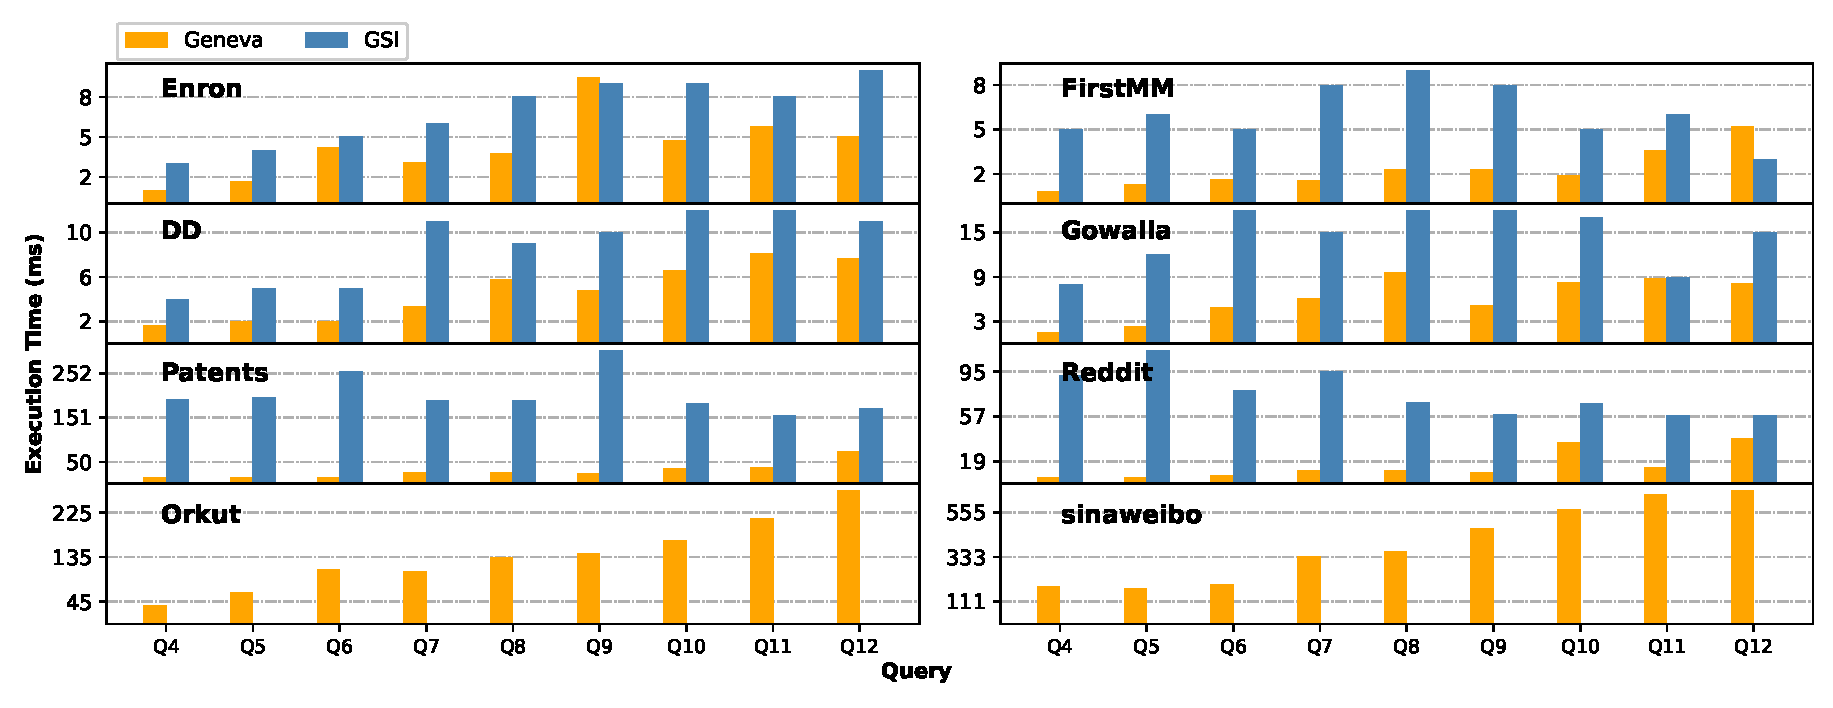
\includegraphics[width=\textwidth]{./figure/overperformance.eps}
\caption{Execution times of \SystemName and GSI for searching nine query graphs on each of eight data graphs.}	
\label{fig:overallperf}
\end{figure*}

\begin{figure}
\centering
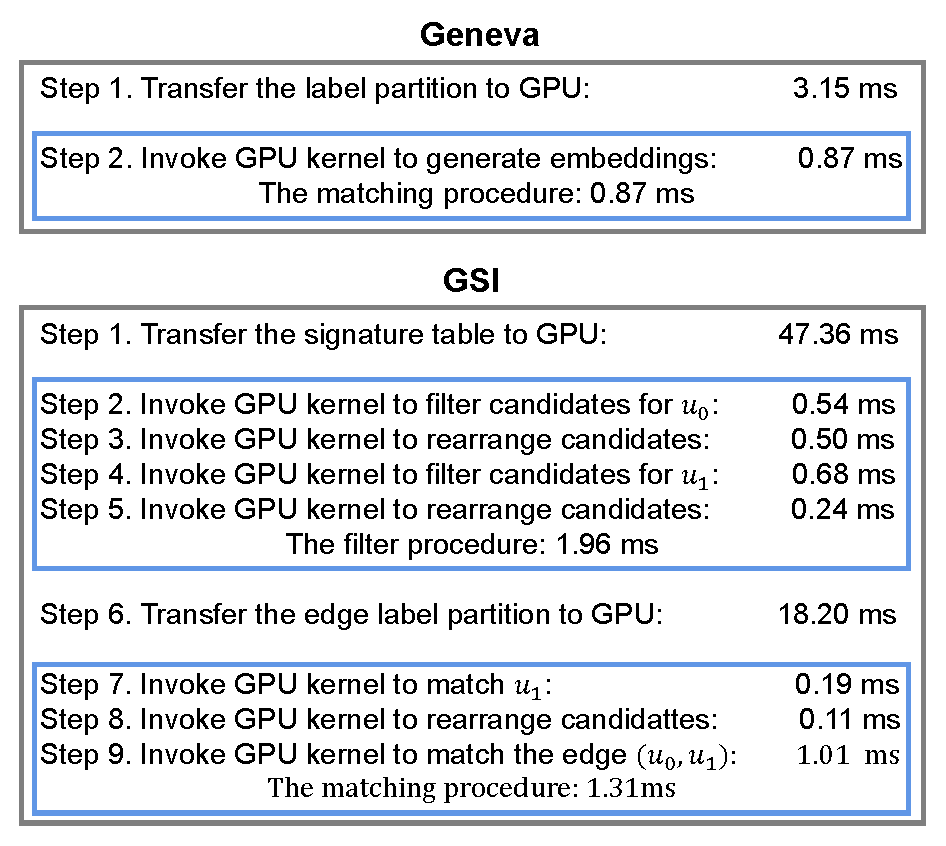
\includegraphics[width=\columnwidth]{./figure/comparegsi.eps}
\caption{The execution times of main procedures of \SystemName and GSI.}	
\label{fig:compdvgsi}
\end{figure}
In this section, we present the overall performance of \SystemName and GSI on eight data graphs. For each data graph, we first use random walk to extract nine query graphs from it with vertex count ranging from 4 to 12, and then employ both methods on the data graph to match the generated nine queries. The runtime results are shown in Fig \ref{fig:overallperf}. GSI runs out of GPU memory in data graphs Orkut and sinaweibo.

Our approach outperforms GSI in almost all test cases and achieves an average speedup of $5\times$. The maximum speedup of our approach over GSI can be up to $22.5\times$. As can be seen, GSI outperforms our approach in two test cases. The reasons can be explained as follows: (1) When matching $Q9$ in the data graph Enron, GSI finds 620K embeddings while \SystemName finds over 19M embeddings. GSI misses a vast number of embeddings, which makes it more faster than \SystemName; (2) When matching $Q12$ in the data graph FirstMM, GSI exits after matching three vertices because no embeddings can be matched, while \SystemName matches all vertices and edges of $Q12$ and finds one embedding. Therefore, \SystemName is slower than GSI in this test case.

In Figure \ref{fig:overallperf}, the average speedup of \SystemName over GSI is $7\times$ for small queries ($Q4$-$Q7$), while it is $3\times$ for large queries ($Q8$-$Q12$). The reason behind this phenomenon is explained as follows. \SystemName can generate an initial extension phase with at least two vertices. Additionally, if there exist vertices that form one of matching patterns 1-4, our approach can generate an initial extension phase with three vertices. Therefore, only two or three extension phases are needed for small queries to complete the matching process. This saves a large number of global memory accesses, which significantly accelerate the matching process for small query graphs.

To find out dominating factors for the superiority of \SystemName over GSI, we analyze detailed runtimes of each procedure of both methods. We employ \SystemName and GSI to match the query graph $Q4$ in the data graph Patents, and present the runtime of each step in Figure \ref{fig:compdvgsi}. We only show runtimes of procedures invoked when matching the first two query vertices, $u_0$ and $u_1$. The reasons are twofold: (1) In GSI, steps after matching $u_0$ and $u_1$ repeat steps 6-9 of Figure \ref{fig:compdvgsi}, and exhibit similar performance; (2) The runtimes of following steps are affected by the number of intermediate embeddings. Only when matching the first two vertices, we can make sure that both \SystemName and GSI process the same number embeddings.

We show the runtimes of \SystemName and GSI in Figure \ref{fig:compdvgsi}, and reveal three root causes of inefficiency of GSI compared to \SystemName.
\begin{itemize}
  \item GSI utilizes a filter procedure to prune candidates for each query vertex. It takes 1.96 ms to complete, which is twice the runtime of the matching procedure of \SystemName. Moreover, GSI needs to transfer the signature table to GPU before running the filter procedure. The runtime of data transfer along takes up 68\% runtime of GSI. This is because the signature table uses 64 bytes for each vertex in the data graph to store neighbor information, which results in a large data structure. Compared to GSI, \SystemName does not employ the filter procedure due to its inefficiencies in time and space.

  \item Before the matching procedure, both methods need to transfer the edge label partition to GPU. However, the execution time of data transfer in GSI is six times slower than \SystemName. The reason is explained as follows. GSI builds a hash-PCSR data structure for each edge label partition and inserts 30 empty entries into hash indexes to reduce the number of collisions. Consequently, hash-PCSR occupies a large portion of memory space, and thus takes a much longer time to be moved to GPU than the interval-PCSR of \SystemName.

  \item In the matching procedure, GSI invokes three GPU kernels to match the query vertex $u_1$, rearrange intermediate embeddings, and match the edge between $u_0$ and $u_1$, respectively. The kernel invoked in step 9 consumes most of the runtime of the matching procedure because it uses multiple time-consuming operations, such as thread block level synchronization and memory copy operations, inside the GPU kernel to maintain load balance. The four-layer load balance scheme of GSI can reduce the load imbalance greatly but also incur significant overhead. Different from GSI, our load balance scheme is simple yet effective. Only when there is no embeddings left, load imbalance can occur.
\end{itemize}

In summary, our approach obtains superior performance over GSI which is the state-of-the-art subgraph matching approach on GPU.

\subsection{Comparison of \SystemName and SV-match} \label{sec:comparesv}
\begin{figure*}
\centering
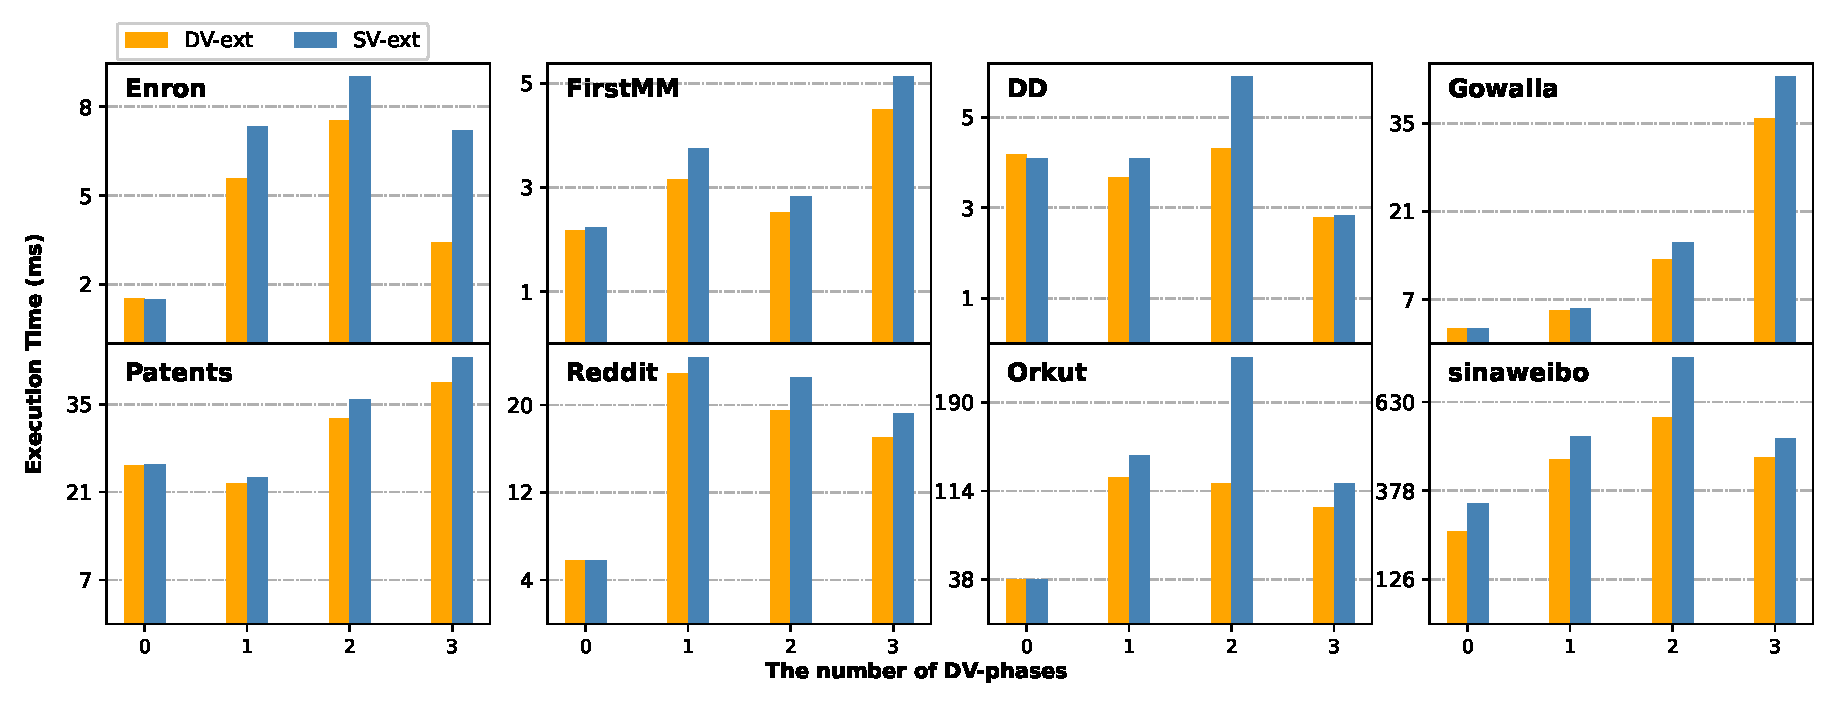
\includegraphics[width=\textwidth]{./figure/compareSV.eps}
\caption{Execution times of \SystemName and SV-match for different number of extension phases that contain matching patterns 1-7.}	
\label{fig:compareSV}
\end{figure*}
To further evaluate the performance of \SystemName, we demonstrate how the number of extension phases that contain matching patterns 1-7 affect the performance of \SystemName. For simplicity, we call the extension phase that contains one of matching patterns 1-7 the PV-phase, and the extension phase that contains the matching pattern 0 the SV-phase. For each data graph, we use random walk to extract several query graphs and classify them into different categories by the number of PV-phase, and select one query graph from each category for each data graph. The results are shown in Figure \ref{fig:compareSV}.

We can see in Figure \ref{fig:compareSV} that when the number of PV-phase is 0, both \SystemName and SV-match exhibit similar performance because all phases of both methods are the same. When the number of pV-phase is 1, 2, and 3, \SystemName improves the performance of SV-match by 11.3\%, 20.2\%, and 16.3\% respectively. In the data graph DD, the performance of \SystemName is very close to SV-match because there is only one embedding that is isomorphic to the query graph and the runtime is too short to observe the difference between \SystemName and SV-match.


\section{Conclusions}
We have presented \SystemName, a GPU-based parallel vertex matching scheme for performing subgraph search in a labeled undirected data
graph. \SystemName is designed to match multiple vertices within a single GPU kernel to reduce the GPU memory accesses. It implements a new
vertex storage format to reduce the memory footprint and vertex search time. We evaluate \SystemName by applying it to eight real-life
graph datasets on an NVIDIDA 2080Ti GPU. We compare \SystemName against GSI, the state-of-the-art GPU-based subgraph search framework.
Experimental results show that \SystemName consistently and significantly outperforms GSI on all test datasets. We also show that our
parallel vertex matching scheme delivers better performance than a variant that implements a single-vertex matching scheme but with our
enhanced storage format.


\bibliographystyle{ACM-Reference-Format}
\bibliography{refs}
\end{document}
\endinput
